%%%%%%%%%%%%%%%%%%%%%%%%%%%%%%%%%%%%%%%%%
% Stylish Article
% LaTeX Template
% Version 2.1 (1/10/15)
%
% This template has been downloaded from:
% http://www.LaTeXTemplates.com
%
% Original author:
% Mathias Legrand (legrand.mathias@gmail.com) 
% With extensive modifications by:
% Vel (vel@latextemplates.com)
%
% License:
% CC BY-NC-SA 3.0 (http://creativecommons.org/licenses/by-nc-sa/3.0/)
%
%%%%%%%%%%%%%%%%%%%%%%%%%%%%%%%%%%%%%%%%%

%----------------------------------------------------------------------------------------
%	PACKAGES AND OTHER DOCUMENT CONFIGURATIONS
%----------------------------------------------------------------------------------------

\documentclass[10pt]{SelfArx} % Document font size and equations flushed left

\usepackage[english]{babel} % Specify a different language here - english by default

\usepackage{lipsum} % Required to insert dummy text. To be removed otherwise

\captionsetup[figure]{justification=justified, singlelinecheck=off} 
\captionsetup[table]{justification=justified, singlelinecheck=off} 

%----------------------------------------------------------------------------------------
%	COLUMNS
%----------------------------------------------------------------------------------------

\setlength{\columnsep}{0.55cm} % Distance between the two columns of text
\setlength{\fboxrule}{0.75pt} % Width of the border around the abstract
\linespread{1.5}

%----------------------------------------------------------------------------------------
%	COLORS
%----------------------------------------------------------------------------------------

\definecolor{color1}{RGB}{0,0,90} % Color of the article title and sections
\definecolor{color2}{RGB}{10,20,20} % Color of the boxes behind the abstract and headings
\definecolor{xsubj}{RGB}{243,194,68} 
\definecolor{xsess}{RGB}{53,99,161} 
\definecolor{xsamp}{RGB}{18,165,121} 

%----------------------------------------------------------------------------------------
%	HYPERLINKS
%----------------------------------------------------------------------------------------

\usepackage{hyperref} % Required for hyperlinks
\hypersetup{hidelinks,colorlinks,breaklinks=true,urlcolor=color2,citecolor=color1,linkcolor=color1,bookmarksopen=false,pdftitle={Title},pdfauthor={Author}}
%----------------------------------------------------------------------------------------
%	ARTICLE INFORMATION
%----------------------------------------------------------------------------------------

% \JournalInfo{Journal, Vol. XXI, No. 1, 1-5, 2013} % Journal information
\JournalInfo{$ $ } % Journal information
\Archive{Pre-print} % Additional notes (e.g. copyright, DOI, review/research article)

\PaperTitle{Perturbation-Enabled Data Augmentation Improves the Generalizability of Classifiers in Network Neuroscience} % Article title

\Authors{Gregory Kiar\textsuperscript{1}, Alan C. Evans\textsuperscript{1}, Tristan Glatard\textsuperscript{2}} % Authors
\affiliation{\textsuperscript{1}\textit{Montréal Neurological Institute, McGill University, Montréal, QC, Canada}}
\affiliation{\textsuperscript{2}\textit{Department of Computer Science and Software Engineering, Concordia University, Montréal, QC, Canada}}

\Keywords{Stability --- Network Neuroscience --- Neuroimaging --- Machine Learning --- Generalizability} % Keywords - if you don't want any simply remove all the text between the curly brackets
\newcommand{\keywordname}{Keywords} % Defines the keywords heading name

%----------------------------------------------------------------------------------------
%	ABSTRACT
%----------------------------------------------------------------------------------------

\Abstract{Machine learning models are commonly applied to human brain imaging datasets in an effort to associate
function or structure with behaviour, health, or other individual attributes. Such models often rely on low-dimensional
maps relating brain regions, generated by complex processing pipelines. However, the numerical instabilities inherent
to pipelines limits the fidelity of these estimates, and results in bias-rich derivatives serving as inputs to these
machine learning models. This work seeks to take advantage of numerical instabilities in pipelines towards reducing the
bias in networks used by machine learning models. We found that resampling brain networks across a series of
numerically perturbed outcomes led to more consistently generalizable performance in all tested classifiers,
preprocessing strategies, and dimensionality reduction techniques when tasked with an age classification task.
Importantly, this finding does not hinge on a large number of perturbed networks in order to exhibit improved
performance, suggesting that even minimally perturbing a dataset reduces bias in the resulting models.}


%----------------------------------------------------------------------------------------

\begin{document}

\flushbottom % Makes all text pages the same height
\maketitle % Print the title and abstract box
% \tableofcontents % Print the contents section
\thispagestyle{empty} % Removes page numbering from the first page

%----------------------------------------------------------------------------------------
%	ARTICLE CONTENTS
%----------------------------------------------------------------------------------------
\pagestyle{fancy}
\section*{Introduction}
\begin{itemize}
\item machine learning has become commonplace for the identification and characterization of individual biomarkers.
\item in neuroimaging, models accept processed imaging data and seek to relate structure or function to phenotypes.
\item the development of biomarkers through this approach has been widely applied, such as linking sex, age, bmi, etc.,
to brain structure.
\item however, these models are sensitive the data used for training, and performance out-of-sample often degrades
significantly.
\item this truth of machine learning is not helped by the fact that bias-rich estimates are used as inputs to the
machine learning models, as scientific pipelines at best provide ``estimates'' of structure or function, rather than
capturing true and unobstructed signal.
\item the impact that numerical instabilities play in determining the results of pipelines have been clearly
demonstrated across operating systems, data perturbations, and pipeline perturbations through MCA
\item a benefit of characterizing instabilities through perturbation approaches is that they result in a series of
estimates of derivatives for each sample in a dataset.
\item here, we take advantage of a range of possible – and equally plausible – outputs from a MCA experiment on
structural connectomes estimation pipeline to augment out dataset.
\item we classify brain networks based on participant age, and resample the samples used for this task based on the
augmented dataset.
\item we evaluate the impact of data augmentation through MCA, explore the relationship between the change in
performance and baseline performance for the classification task, and identify any relationship between these potential
benefits and the number of MCA simulations performed per sample.
\end{itemize}

\section*{Materials \& Methods}

The objective of this study was to evaluate the impact of aggregating collections of unstable brain networks towards
learning robust brain-phenotype relationships. We sampled and aggregated simulated networks within individuals to learn
relationships between brain connectivity and individual an trait, in this case age, and compared this to traditional
baseline performance on this tasks. We compared aggregation strategies with respect to baseline validation performance,
performance out-of-sample, and generalizability.

All developed software and analysis resources for this project have been made available through GitHub at
\url{https://github.com/gkpapers/2020AggregateMCA}.

\subsection*{Dataset}

An existing dataset containing Monte Carlo Arithmetic (MCA) perturbed structural human brain networks was used for
these experiments~\cite{Kiar2020-yz}. The perturbations introduced for the generation of brain networks in this dataset
were at the level of machine-error, simulating expected error over a typical pipeline execution. This dataset contains
a single session of data from $100$ individuals ($100\times 1 \times1$). The derived brain networks were generated with
a probabilistic structural connectome estimation pipeline~\cite{Garyfallidis2014-ql} using a fixed random seed, and
Monte Carlo Arithmetic (MCA) perturbations were added to all Python-implemented operations throughout the
pipeline~\cite{Denis2016-wo,Parker1997-qq}. Each sample was simulated $20$ times, resulting in $2,000$ unique graphs.
Further information on the processing and curation of this dataset can be found here~\cite{Kiar2020-kz}.

This collection enabled the exploration of subsampling and aggregation methods in a typical learning context for
neuroimaging~\cite{Dimitriadis2017-pd,Buchanan2014-pm}. Exploring the relationship between the number of simulations
and performance further allows for MCA-enabled resampling to be evaluated as a method of dataset augmentation.

As the target for classification, individual-level phenotypic data strongly implicated in brain connectivity was
desired. Participant age, which has consistently been shown to have a considerable impact on brain
connectivity~\cite{Meier2012-ve,Wu2012-uc,Bookheimer2019-ti,Zhao2015-rm}, was selected and turned into a binary target
by dividing participants into adult ($>18$) and non-adult groups ($68\%$ adult).

\subsection*{Preprocessing}
Prior to being used for this task, the brain networks being were represented as symmetric $83 \times 83$ adjacency
matrices, sampled upon the Desikan-Killiany-Tourville~\cite{Klein2012-vi} anatomical parcellation. To reduce redundancy
in the data, all edges belonging to the upper-triangle of these matrices were preserved and vectorized, resulting in a
feature vector of $3,486$ edges per sample. All samples were preprocessed using one of four standard techniques:

\paragraph{Raw} The raw streamline count edge-weight intensities were used as originally calculated.

\paragraph{Log Transform} The log10 of edge weights were taken, and edges with $0$ weight prior to the transform were
reset to $0$.

\paragraph{Rank Transform} The edges were ranked based on their intensity, with the largest edge having the maximum
value. Ties were settled by averaging the rank, and all ranks were finally min-max scaled between $0$ and $1$.

\paragraph{Z-Score} The edge weights were z-scored to have a mean intensity of $0$ and unit variance.

\subsection*{Machine Learning Pipelines}

The preprocessed connectomes were fed into pipelines consisting of two steps: dimensionality reduction and
classification. Dimensionality reduction was applied using one of two methods:

\paragraph{Principal Component Analysis} The connectomes were projected into the $20$ dimensions of highest variance.
The number of components was chosen to capture approximately $90\%$ of the variance present within the dataset.

\paragraph{Feature Agglomeration} The number of features in each connectome were reduced by combining edges according
to maximum similarity/minimum variance using agglomerative clustering~\cite{Ward1963-uh}. The number of resulting
features was $20$, to be consistent with the number of dimensions present after PCA, above.

After dimensionality reduction, samples were fed into one of five distinct classifiers as implemented through scikit
learn~\cite{Pedregosa2011-uz}:

\paragraph{Support Vector Machine} The model was fit using a radial basis function (RBF) kernel, L2 penalty, and a
balanced regularization parameter to account for uneven class membership.

\paragraph{Logistic Regression} A linear solver was used due to the relatively small dataset size. L2 regularization
and balanced class weights were used, as above.

\paragraph{K-Nearest Neighbour} Class membership was determined using an L2 distance and the nearest $10\%$ of
samples, scaling with the number of samples used for training.

\paragraph{Random Forest} $100$ decision trees were fit using balanced class weights, each splitting the dataset
according to a maximum of $4$ features per node (corresponding to the rounded square root of $20$ total features).

\paragraph{AdaBoost} A maximum of $50$ decision trees were fit sequentially such that sample weights were iteratively
adjusted to prioritize performance on previously incorrectly-classified samples, consistent with~\cite{Freund1997-qy}.

The hyperparameters for all models were refined from their default values to be appropriate for a small and imbalanced
dataset. The performance for all pipeline combinations of preprocessing methods, dimensionality reduction techniques,
and models using the reference (i.e. unperturbed) executions in the dataset ranged from an F1 score of $0.64 – 0.875$
with a mean of $0.806$; this evaluation was performed on a consistent held-out test set which was used for all
experiments, as described in a following section. This set of models was chosen as it includes i) well understood
standard techniques, ii) both parametric and non-parametric methods, iii) both ensemble and non-ensemble
methods, and iv) models which have been commonly deployed for the classification neuroimaging
datasets~\cite{Meier2012-ve,Tunc2016-cz, Zhu2018-cs,Payabvash2019-tm,Crossley2014-tg,Park2015-uj,Nayak2016-wl,Tolan2018-nq}.

\subsection*{Dataset Sampling}

A chief purpose of this manuscript involves the comparison of various forms of aggregation across
equivalently-simulated pipeline outputs. Accordingly, the dataset was resampled prior to dimensionality reduction and
classifiers were trained, evaluated, and combined according to the following procedures:

\paragraph{Reference} Networks generated without any MCA perturbations were selected for input to the models, serving
as a benchmark.

\paragraph{Jackknife} The datasets were repeatedly sampled such that a single randomly chosen observation of each
unique network was selected (i.e. derived from the same input datum). This resampling was performed $100$ times,
resulting in the total number of resamplings being $5\times$ larger than the number of unique observations per network,
ensuring a broad and overlapping sampling of the datasets.

\paragraph{Median} The edgewise median of all observations of the same network were used as the samples for training
and evaluation.

\paragraph{Mean} Similar to the above, the edgewise mean of all observations for each network were computed and used
as input data to the classifiers in both collections.

\paragraph{Consensus} A distance-dependent average network~\cite{Betzel2018-eo} was computed across all observations
of each network. This data-aware aggregation method, developed for structural brain network analysis, preserves network
properties often distorted when computing mean or median networks.

\paragraph{Mega-analysis} All observations of each network were used simultaneously for classification, increaseing
the effective sample size. Samples were organized such that all observations of the same network only appeared within a
single fold for training and evaluation, ensuring double-dipping was avoided.

\paragraph{Meta-analysis} Individual classifiers trained across jackknife dataset resamplings, above, were treated as
independent models and aggregated into an ensemble classifier. The ensemble was fit using a logistic regression
classifier across the outputs of the jackknifed classifiers to learn a relationship between the predicted and true
class labels.

The robustness and possible benefit of each subsampling approach was measured by evaluation on a subset of all MCA
simulations, including $9$ distinct numbers of simulations, ranging from $20$ to $2$ simulations per sample. Combining
the dataset sampling methods, the set of simulations, preprocessing strategies, dimensionality reduction techniques,
and classifier models, there were $2,200$ models trained and evaluated.

\subsection*{Training \& Evaluation}

Prior to training models on the brain networks, $20\%$ of subjects were excluded from each dataset for use as an
out-of-sample test dataset for all experiments. With the remaining $80\%$ of subjects, cross validation was performed
following a stratified grouped $k$-fold approach ($k=5$). In this approach, samples were divided into training and
validation sets such that the target variable was proportionally represented on each side of the fold (stratified),
conditional upon all observations from the same individual, relevant for the mega-analysis dataset sampling method,
falling upon the same side of the fold (grouped). This resulted in $5$ fold-trained classifiers per configuration, each
trained on $64\%$ of the samples and validated on $16\%$, prior to each being tested on the remaining $20\%$ of
held-out samples. All random processes used in determining the splits used the same seed to remove the effect of random
sampling.

Classifiers were primarily evaluated on both the validation and test (out-of-sample) sets using F1 score, a standard
measure for evaluating classification performance. The generalizability of predictions was defined as:

\begin{equation}
G = 1 - \lvert F1_{test} - F1_{validation} \rvert
\label{eq:gen}
\end{equation}

where a score of $1$ (maximum) indicates the equivalent performance across both the validation and test sets, and a
lower score (minimum of $0$) indicates inconsistent performance. The absolute change in performance was used in
Eq.~\ref{eq:gen}, resulting in a score which penalizes spurious over-performance similarly to under-performance, as all
inconsistency is undesirable when applying a classifier out-of-sample.

Differences in F1 score and Generalizability were used to measure the change in performance between the reference and
other dataset sampling techniques, and statistical comparisons were made through Wilcoxon Signed-Rank Tests.


%------------------------------------------------
\section*{Results}

\begin{figure*}[tbh!]\centering
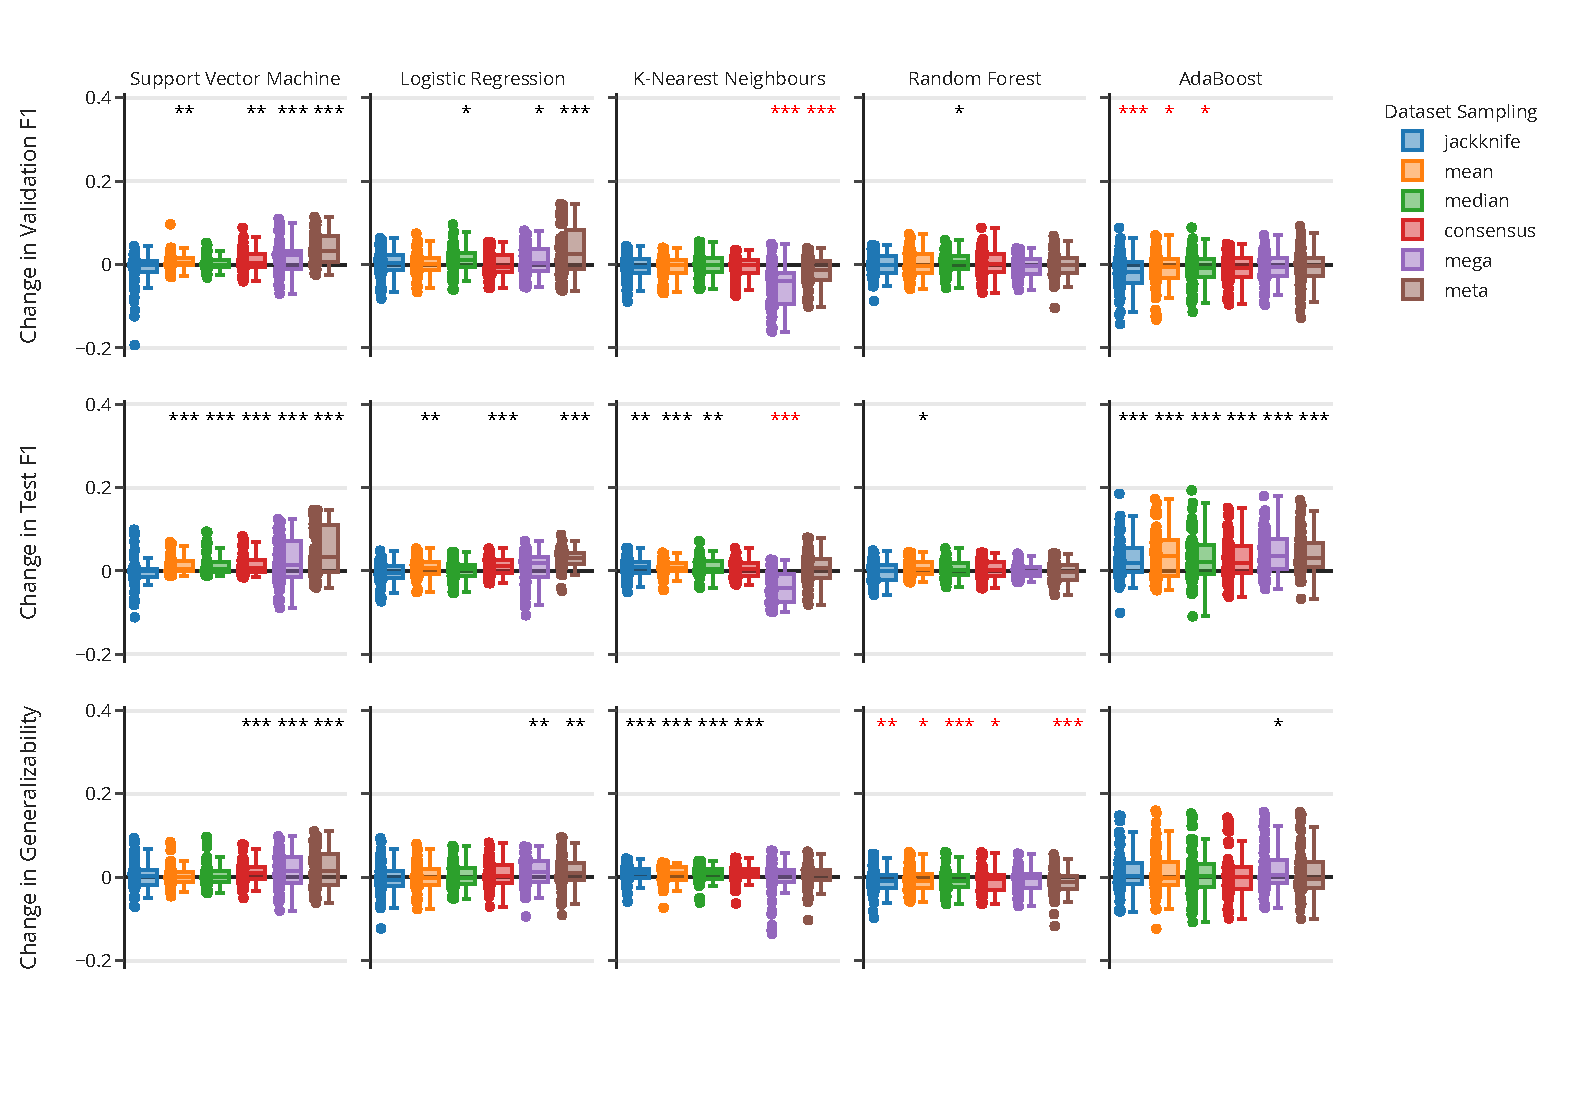
\includegraphics[width=\linewidth]{figures/1.pdf}
\caption{Relative change in classifier performance with respect to classifier type and dataset sampling strategies as
measured by change in F1 score on the validation set (top) or test set (middle), as well as the generalizability of
performance (bottom). Each star annotation indicates an order of magnitude of statistically significant change,
beginning at $0.05$ for one star and decreasing from there, with those in black or red indicating an increase or
decrease due to resampling, respectively.}
\label{fig:overall_perf}
\end{figure*}

The figures and findings presented in this section represent a summary of the complete experiment table which consists
of performance measures and metadata for all $2,200$ models tested. The complete performance table alongside the table
of significant differences, are made available through the GitHub repository.

\subsection*{Data Resampling Improves Classification}

The change in performance for each model and dataset sampling technique is shown in Figure~\ref{fig:overall_perf}. The
change in performance was measured as a change in F1 score on the validation set, the change in F1 score on the test
set, and the change in overall generalizability, a measure which summarizes the similarity between validation and test
performance for a given model.

The support vector machine and logistic regression models improve across each of these three measures for a variety of
dataset sampling techniques, meaning that the addition of the MCA-perturbed samples improves the training, testing, and
overall generalizability of the classifiers.

\begin{figure*}[bht!]\centering
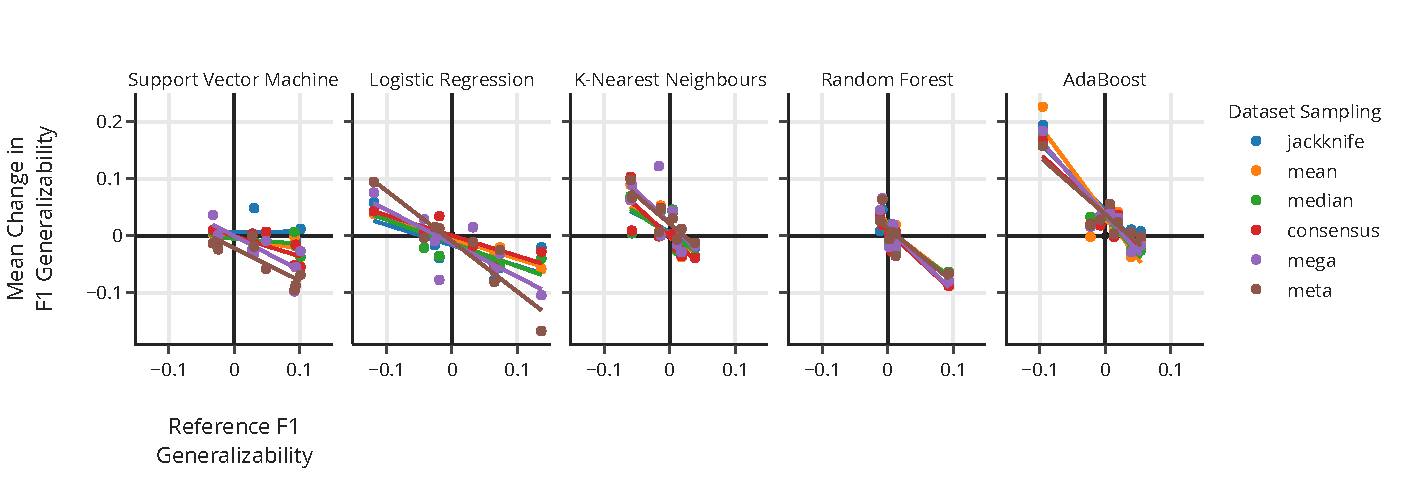
\includegraphics[width=\linewidth]{figures/2.pdf}
\caption{Change in the generalizability of classifiers with respect to the reference generalizability. Each data point
represents the mean change in generalizability for all models using the same preprocessing and dimensionality
reduction techniques for a given classifier and dataset sampling strategy.}
\label{fig:change_in_gen}
\end{figure*}

Distinctly, k-nearest neighbours (KNN) and AdaBoost classifiers experience minimal change in validation and often see
their perfomance decline. However, the improvement of these classifiers on the test set suggests that resampling
reduced overfitting in these classifiers. In the case of KNN, this translates to imrpoved generalizability, while in
the case of AdaBoost generalizability was largely unchanged, suggesting that the model went from underperforming to
overperforming after dataset resampling. The unique decline in performance when using the mega-analytic resampling
technique on KNN classifier is suggestive of poor hyperparameterization, as there is a strong relationship between the
number of samples in the dataset and the $k$ parameter of the model. At present this parameter was scaled linearly with
the number of MCA simulations used, however, it is both possible that an improved scaling function exists or that the
model performance degrades with large sample sizes making it a poor model choice given this resampling technique.

The random forest classifiers uniquely did not see a significant change in validation or testing performance across the
majority of resampling techniques. However, these classifiers did experience a significant decrease in the
generalizability of their performance, meaning that there was a larger discrepancy between training and testing
performance in many cases. This distinction from the other models is likely due to the fact that random forest is a
simple ensemble technique which takes advantage of training many independent classifiers and samples them to assign
final class predictions. It is likely that this approach forms more generalizable predictions generally, and thus the
addition of more data does not improve performance further. While AdaBoost is also an ensemble method, the iterative
training of models based on sample difficulty allows for the added variance in those samples to play an increasingly
central role in the construction of class relationships.

Across all classifier types, it was found that both mega- and meta-analytic approaches outperformed other methods
slightly, though this was not statistically significant. Additionally, while certain combinations of preprocessing,
dimensionality reduction, and classifiers performed more harmoniously than others, there was no significant
relationship between the performance of any single resampling method and preprocessing or dimensionality reduction
technique. The above results show that dataset augmentation through MCA-perturbed pipeline outputs may be an effective
way to improve the performance and generalizability of non-ensemble classifiers tasked with modeling brain-phenotype
relationships, both within and out of sample.

\subsection*{Model Improvement Scales With Generalizability}

\begin{itemize}
\item Perturbation-enabled dataset resampling improves generalizability
\item Less generalizable models improve more
\item With the excecption of KNN, for which all models already exhibited high performance, there was a significant
relationship between the baseline generalizability and the improvement from perturbations.
\item The models which decrease in generalizability all have high generalizability scores ($>0.935$), and this is
likely the paired result of "removing good luck" while the other is "removing bad luck"
\end{itemize}


\subsection*{Mega-Analysis Improves With Samples}

\begin{figure*}[ht]\centering
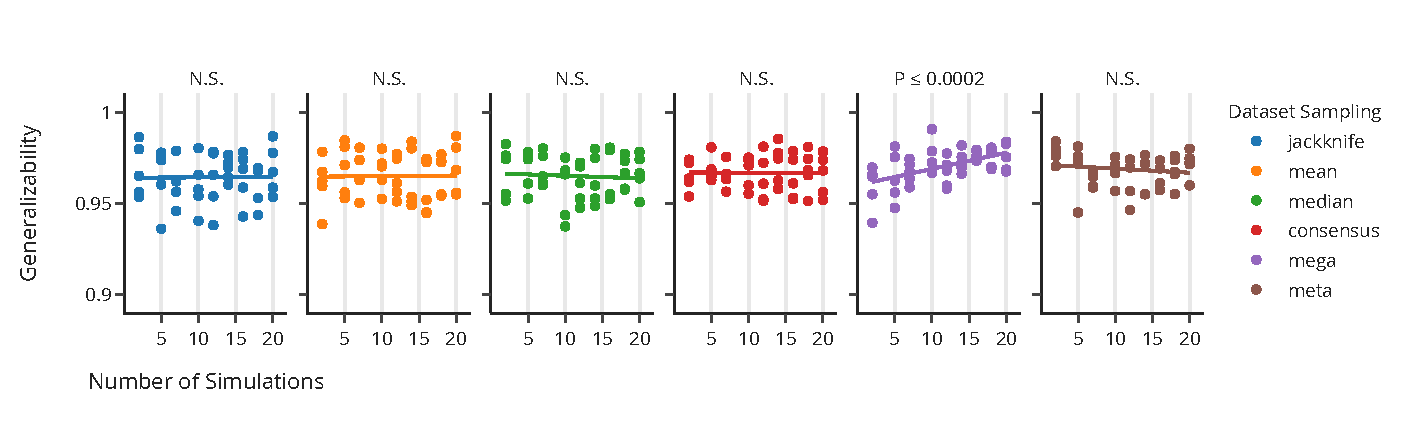
\includegraphics[width=\linewidth]{figures/3.pdf}
\caption{The generalizability of classifiers using each dataset sampling technique with respect to the number of MCA
simulations. Each number of simulations was sampled a single time, to avoid artificial skewing of the dataset due to
the inclusion of ``higher'' or ``lower'' quality samples; a single drawing of each split mimics a true perturbation
experiment context.}
\label{fig:nsamples}
\end{figure*}

\begin{itemize}
\item While we previously note an increase in the generalizability when resampling, there is no relationship between
the number of independent samples used and performance in most cases,
\item however, in the case of the mega-analytic approach, there is a significant relationship between the number of
samples used and generalizability.
\item mega is the only approach that changes the number of samples being used by the classifiers, and this relationship
is consistent to an increase one would expect when increasing the number of samples in their experiment.
\end{itemize}

\section*{Discussion}

\begin{itemize}
\item MCA augmentation is a good thing for performance, increasing our ability to train, test, and generalize
performance in standard models.
\item RF models benefitted the least from MCA, likely because they already combine a series of simple and independent
representations towards making their decisions.
\item Adaboost performance increased dramatically on the testing dataset, however, the lack of generalizability
increase suggests the model went from underperforming to overperforming with the addition of MCA.
\item learning is typically easier in a balanced class setting, and MCA could potentially be used as an oversampling
method to increase the balance of datasets. The advantages of an approach like this are that all results are
biologically plausible, and it would be possible in context when simulation methods specific to the data modality or
processing technique are unavailable.
\item While our work demonstrates that poorer performing classifiers benefit more from this resampling, the limit
of that is unclear. An avenue for future work includes exploring the performance space more broadly, and identifying a
relationship between baseline performance and impact of perturbation-based augmentation. It is unlikely that a model
classifying with an F1 score of $0.95$ would benefit the same as one with $0.75$, or one performing near chance.
\item Further work should situate this result relative to increased data collection. This was not performed here,
despite the existence of an MCA-perturbed repeated-measures dataset in the previous study, as the sample size of $25$
individuals was too small to meaningfully train and evaluate models in a paradigm consistent with other evaluatiions.
\item This work demonstrates the benefit of performing perturbation experiments goes beyond stability evaluation, and
that these methods support data augmentation strategies that significantly improve our ability to model
brain-phenotype relationships.
\end{itemize}

\subsection*{Data \& Code Availability}
The perturbed connectomes were publicly available data resource previously produced and made available by the
authors~\cite{Kiar2020-yz}. They can be found persistently at \url{https://doi.org/10.5281/zenodo.4041549}, and are
made available through The Canadian Open Neuroscience Platform (\url{https://portal.conp.ca/search}, search term
"Kiar"). All software developed for processing or evaluation is publicly available on GitHub at
\url{https://github.com/gkpapers/2020AggregateMCA}. Experiments were launched on Compute Canada's HPC cluster
environment. 

\subsection*{Author Contributions}
GK was responsible for the experimental design, data processing, analysis, interpretation, and the majority of writing.
All authors contributed to the revision of the manuscript. TG and ACE contributed to experimental design, analysis,
interpretation. The authors declare no competing interests for this work. Correspondence and requests for materials
should be addressed to Gregory Kiar at \url{gregory.kiar@mail.mcgill.ca}.

\subsection*{Acknowledgments} 
This research was financially supported by the Natural Sciences and Engineering Research Council of Canada (NSERC)
(award no. CGSD3-519497-2018). This work was also supported in part by funding provided by Brain Canada, in partnership
with Health Canada, for the Canadian Open Neuroscience Platform initiative.

%----------------------------------------------------------------------------------------
%	REFERENCE LIST
%----------------------------------------------------------------------------------------
% \phantomsection
\bibliographystyle{IEEEtran}
\bibliography{aggregating-unstable-derivatives}


\end{document}
